\chapter[The LHC and the ATLAS detector][The LHC and the ATLAS detector]{The LHC and the ATLAS detector}
\label{chap:lhcatlas}

\begin{quote}
  The LHC and ATLAS detector are described.
\end{quote}
 
\section{The LHC}
\label{sec:lhc}

\begin{figure}[tp]
  \centering
  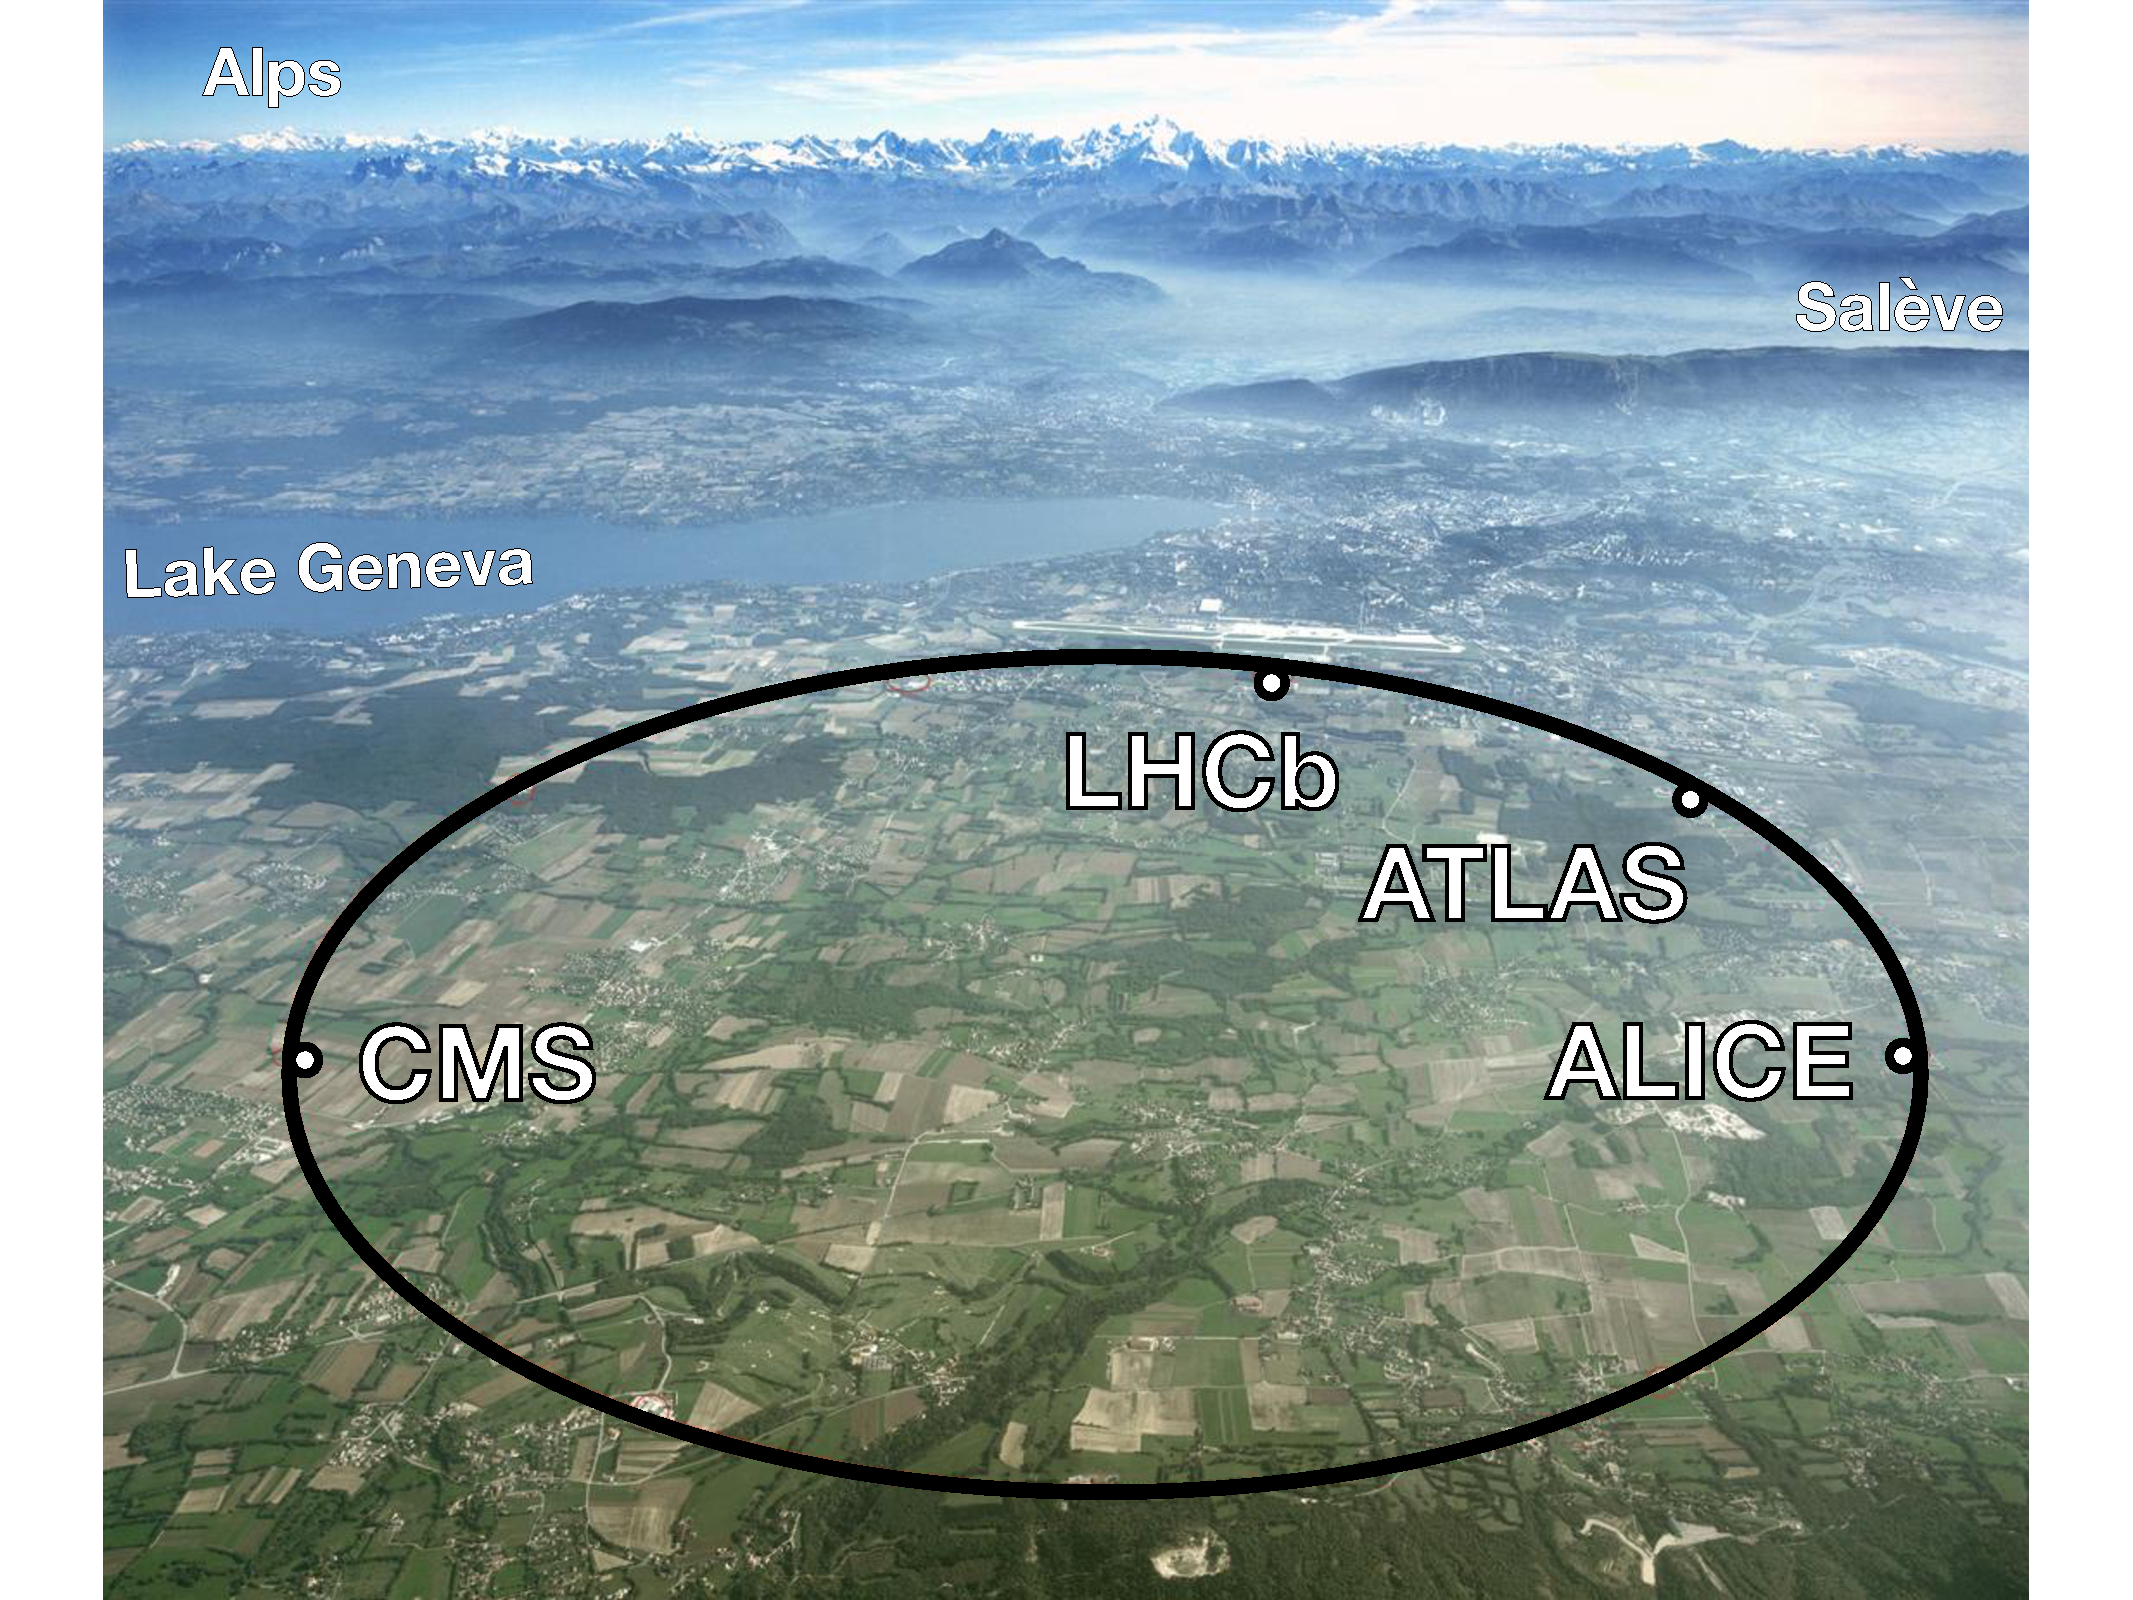
\includegraphics[width=0.90\textwidth]{figures/lhc-atlas/lhc-switzerland}
  \caption{Variables.}
  \label{fig:lhc-switzerland}
\end{figure}

\begin{figure}[tp]
  \centering
  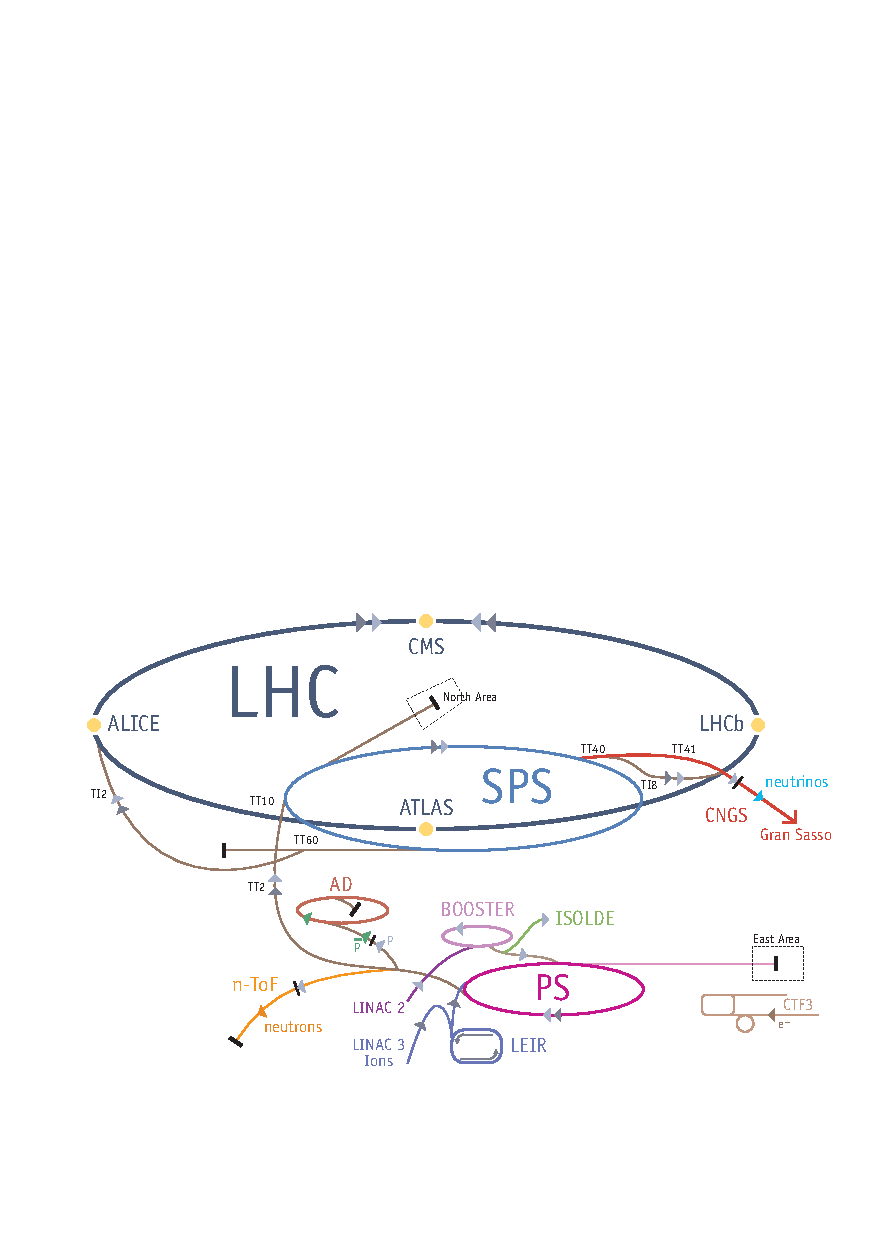
\includegraphics[width=0.90\textwidth]{figures/lhc-atlas/lhc-accelerator-complex}
  \caption{Variables.}
  \label{fig:lhc-complex}
\end{figure}

\begin{figure}[tp]
  \centering
  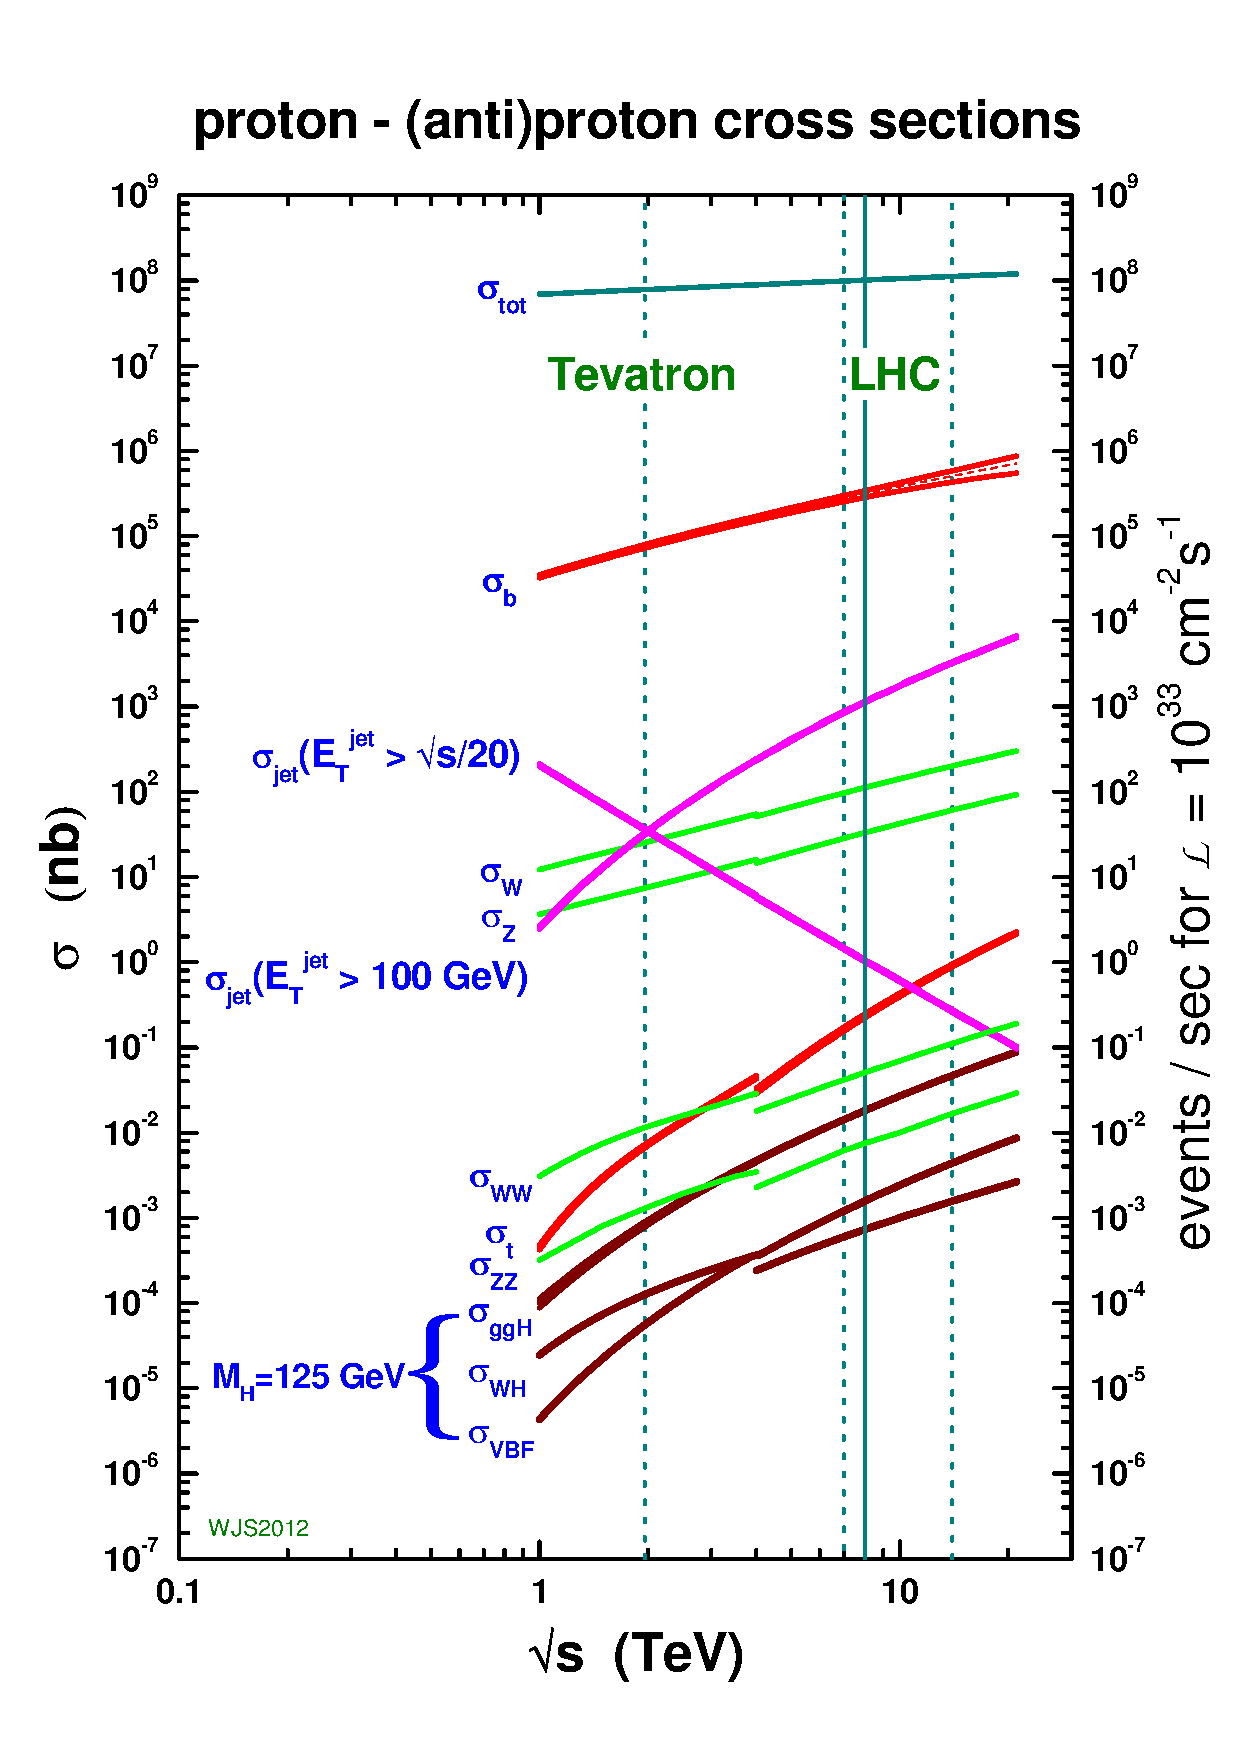
\includegraphics[width=0.90\textwidth]{figures/lhc-atlas/crosssections2012_v5}
  \caption{Variables.}
  \label{fig:lhc-stirling}
\end{figure}

\section{The ATLAS detector}
\label{sec:atlas}

\begin{figure}[tp]
  \centering
  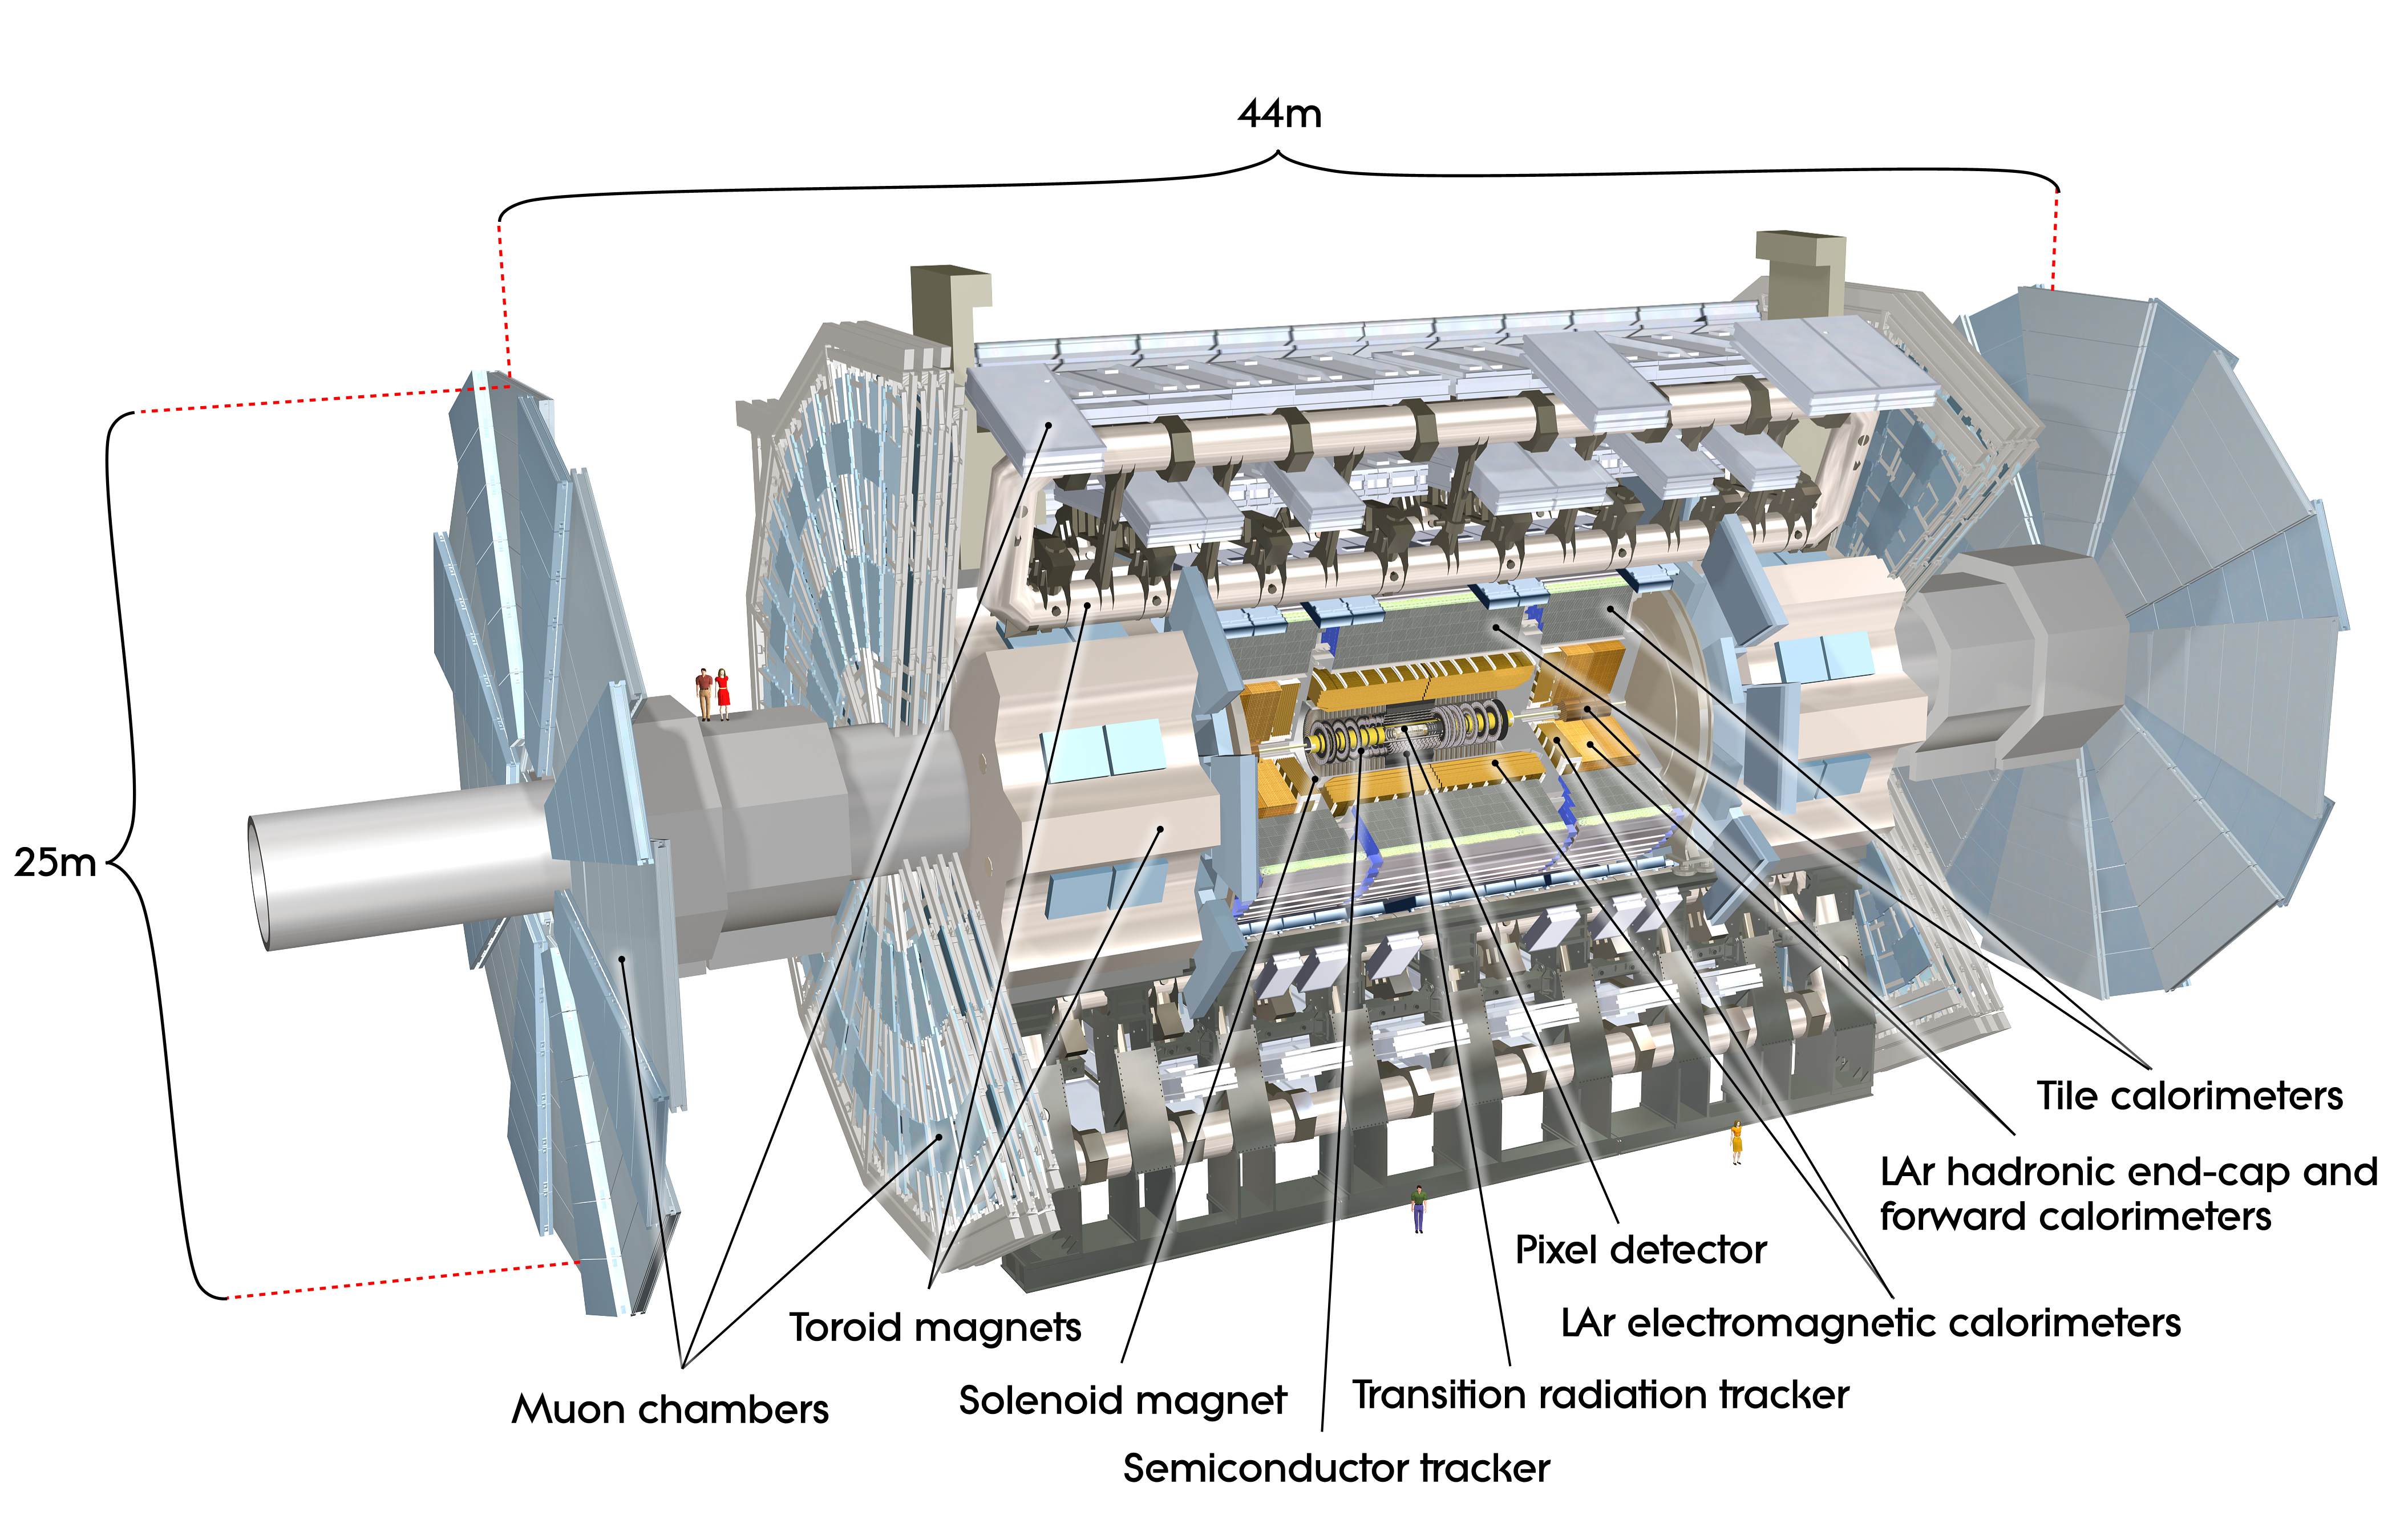
\includegraphics[width=0.90\textwidth]{figures/lhc-atlas/atlas-0803012_01.jpg}
  \caption{Variables.}
  \label{fig:atlas-cartoon}
\end{figure}

\begin{figure}[tp]
  \centering
  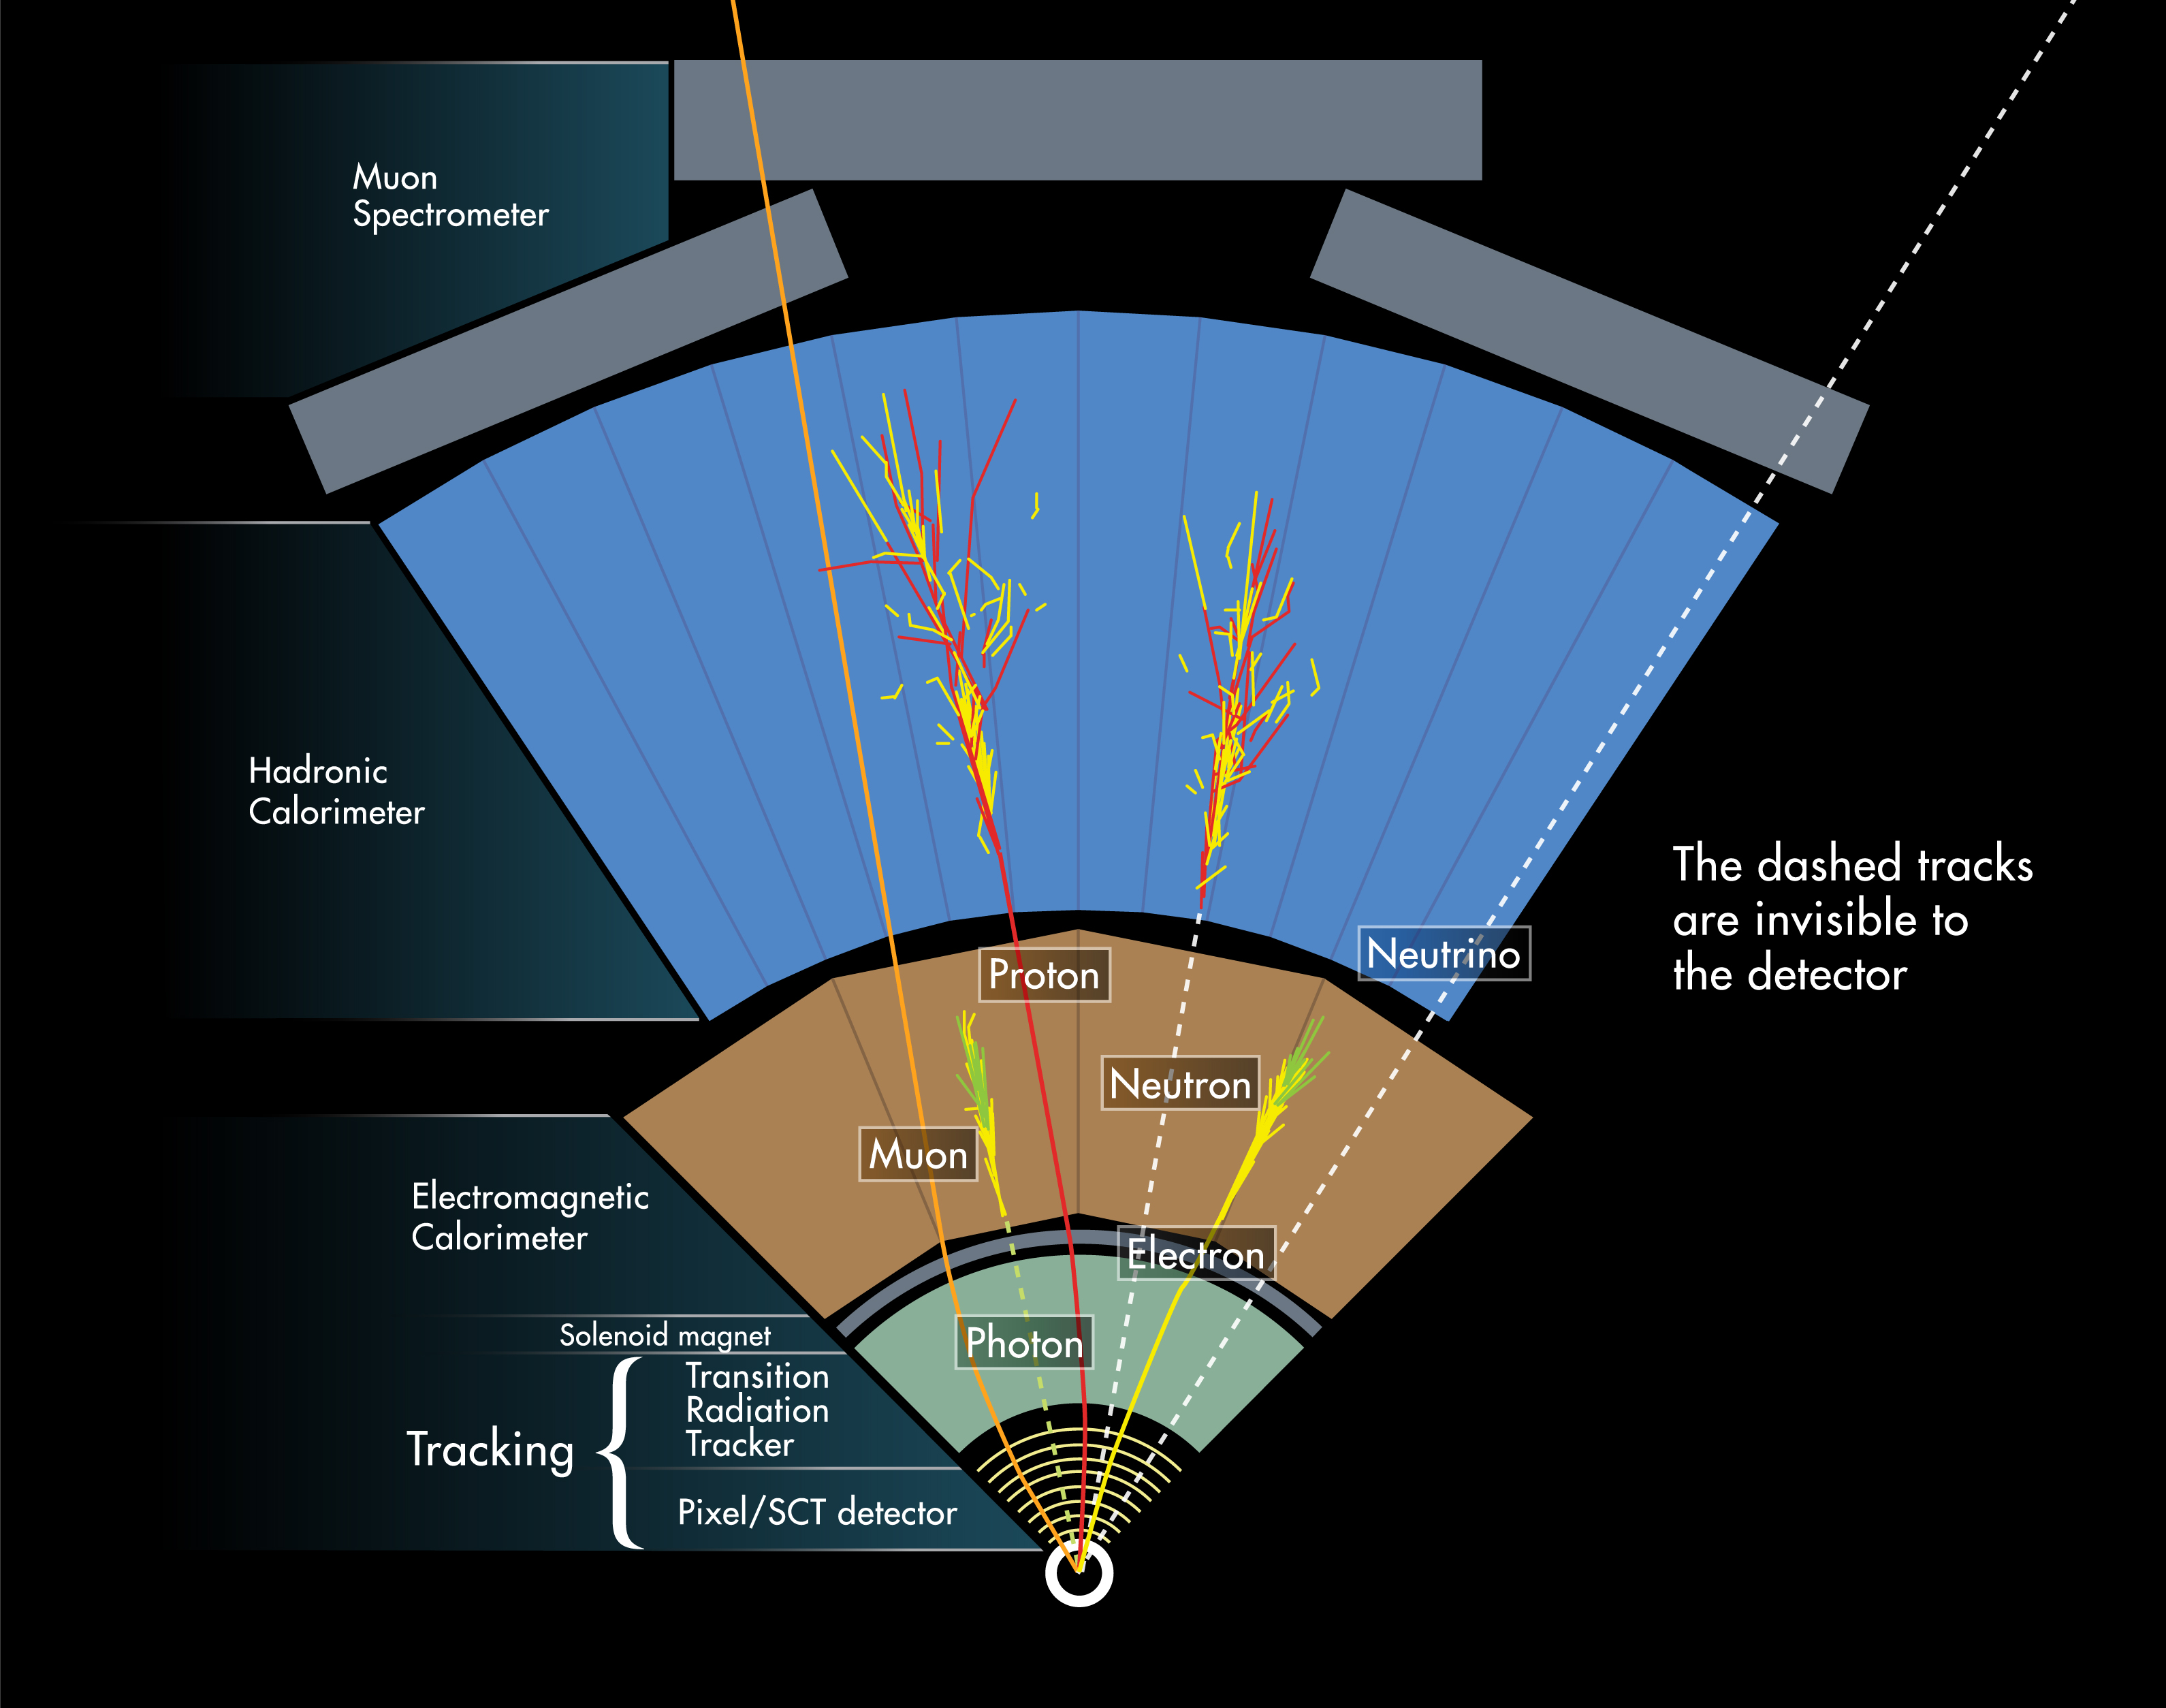
\includegraphics[width=0.90\textwidth]{figures/lhc-atlas/atlas-wedge-1301009_01.jpg}
  \caption{Variables.}
  \label{fig:atlas-wedge}
\end{figure}

\begin{figure}[tp]
  \centering
  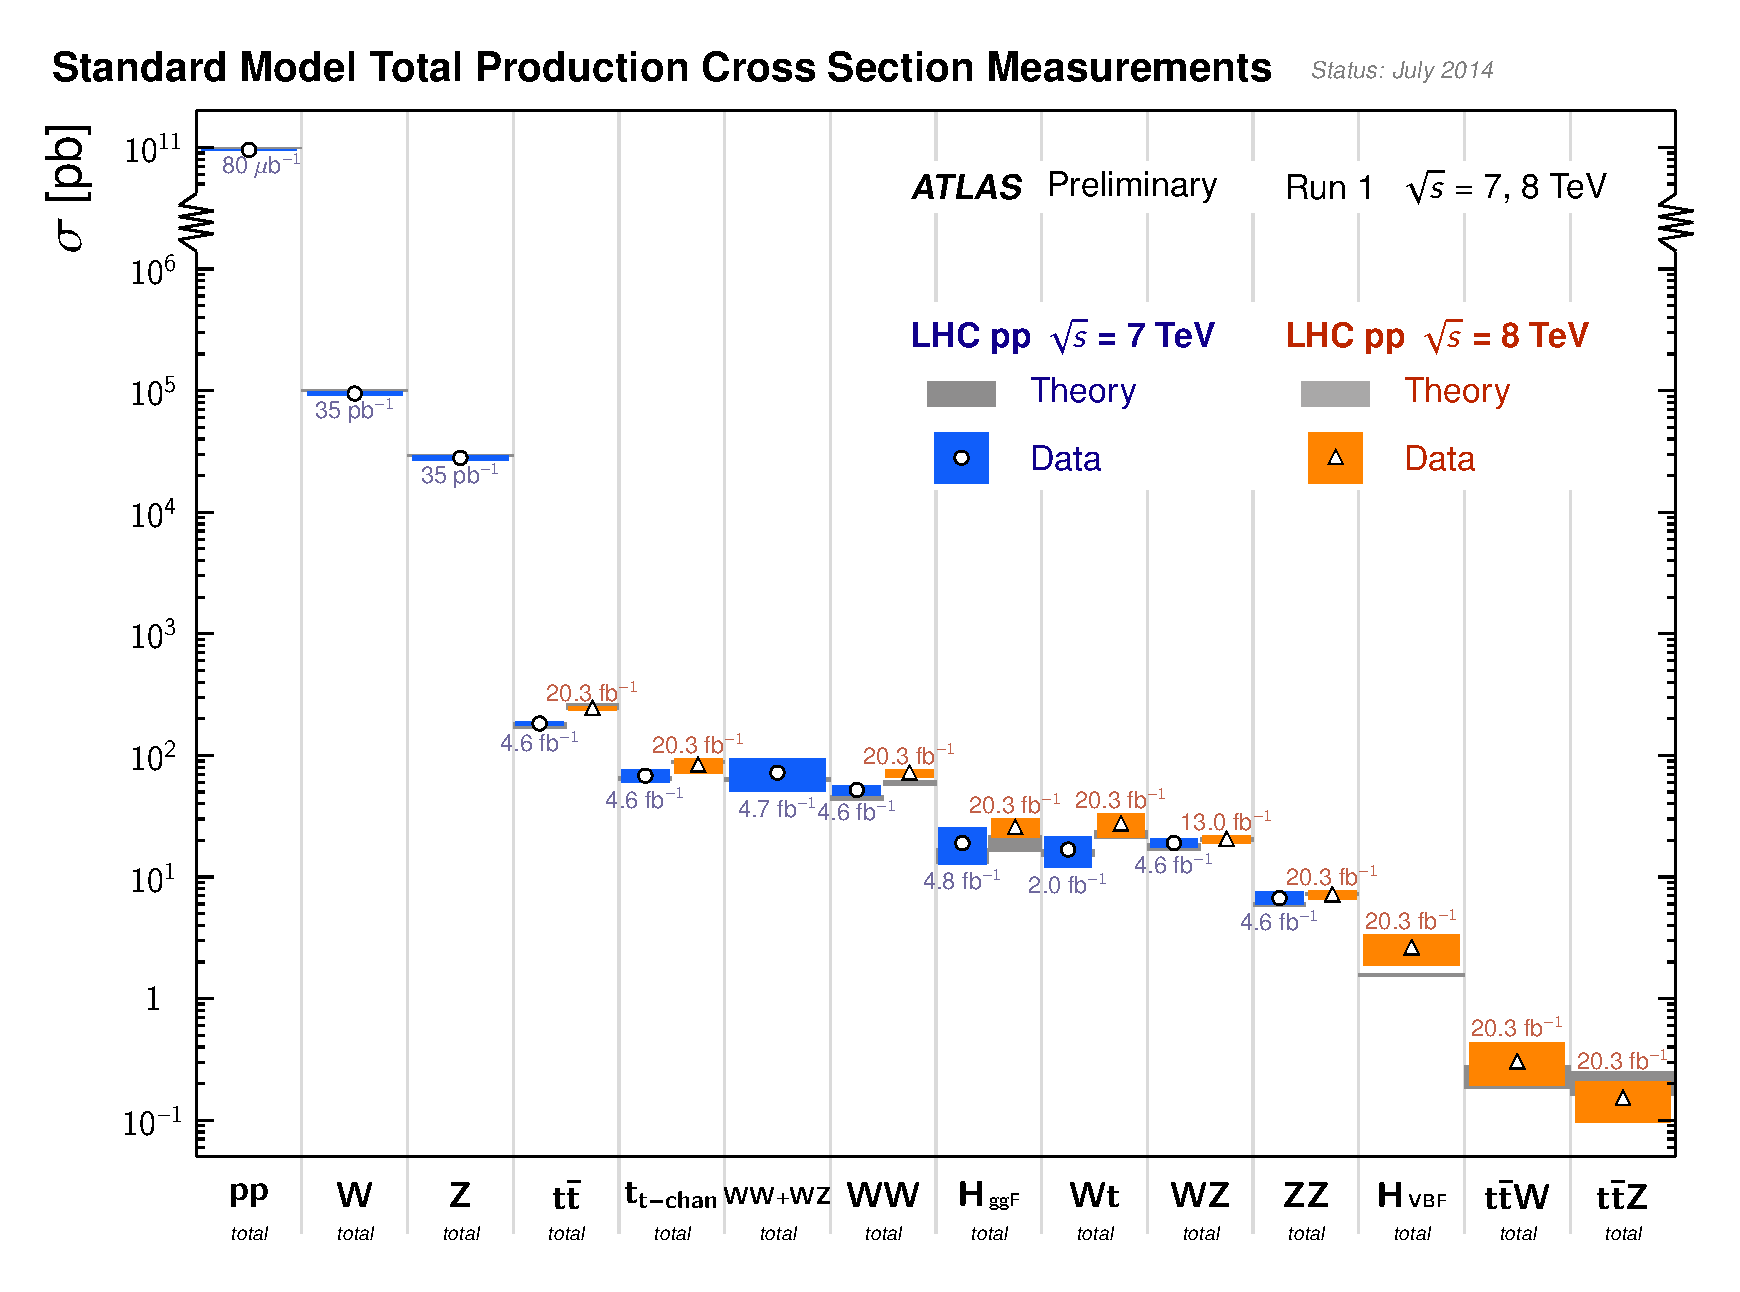
\includegraphics[width=0.90\textwidth]{figures/lhc-atlas/ATLAS_a_SMSummary_TotalXsect}
  \caption{Variables.}
  \label{fig:atlas-measurements}
\end{figure}

\section{Tracking}
\section{Calorimetry}
\section{Muon spectrometry}
\section{Particle identification}
\subsection{Muons}
\subsection{Electrons and photons}
\subsection{Hadrons}
\subsubsection{Jets}
\subsubsection{Jets from $b$-hadron decays}
\subsubsection{Jets from $\tau$ lepton decays}
\subsection{Neutrinos}
\section{Triggering}


